\documentclass[conference]{IEEEtran}
\usepackage{amsmath,amssymb,booktabs,graphicx,microtype}
\title{Constraint-Aware Candidate-Set MAPPO for Stable Routing in Dynamic LEO Networks}
\author{\IEEEauthorblockN{Author information to be inserted before submission}}
\begin{document}
\maketitle

\begin{abstract}
Low-Earth-orbit routing policies must react to topology and congestion without
changing cached next hops unnecessarily. We formulate decision-level avoidable
switching as a constrained objective for a distributed candidate-set MAPPO
policy. A permutation-equivariant actor scores feasible neighbors while a
graph critic and centered local credit are used only during centralized
training. The controller enforces a 0.12 avoidable-switch-rate budget through
a learned dual variable. In a preregistered sealed test with two dynamic
24-satellite scenarios, eight independently trained policy seeds, and 50
paired unseen workloads, the constrained policy reduced the avoidable-switch
rate by 15.22 and 36.25 percentage points. Delivery was non-inferior within a
prespecified two-percentage-point margin: the effects were -0.96 points under
medium load and +0.77 points under hotspot load. All integrity, budget,
rate-reduction, and delivery gates passed. The results support a bounded claim
that explicit decision-level constraints can trade small delivery changes for
substantial routing stability in the audited simulator.
\end{abstract}

\section{Introduction}
LEO satellite networks expose routing agents to moving connectivity, link
failures, queue imbalance, and changing traffic concentrations. A policy that
maximizes delivery alone may repeatedly replace a still-feasible cached next
hop. Such churn complicates forwarding-state maintenance and can amplify
control overhead. Conversely, a rigid shortest-path policy can ignore local
congestion.

We study distributed next-hop selection with centralized training and local
execution. The operational endpoint is a \emph{decision-level avoidable
switch}: the cached next hop and an alternative are both feasible, yet the
policy chooses a different neighbor. This is distinct from a forced switch
after link failure and from end-to-end route recomputation.

Our contributions are: (i) a masked, permutation-equivariant candidate-set
actor for dynamic local connectivity; (ii) an explicit constrained MAPPO
objective that targets an auditable avoidable-switch-rate budget; and (iii) a
sealed, seed-level paired evaluation with exact randomization tests and crossed
bootstrap intervals. MAPPO itself is not claimed as novel.

\section{Related Work}
Snapshot shortest-path and virtual-topology schemes remain central to LEO
routing, while Q-routing adapts next hops from local delay feedback
\cite{boyan1994q}. Hypatia enables packet-level evaluation over realistic
constellation traces \cite{klenze2020hypatia}. Learning-based routing adds
adaptation but often reports episode replications as independent or leaves
route churn implicit. Our actor follows set-function symmetry principles
\cite{zaheer2017deepsets} and invalid-action masking, while centralized
training follows PPO/MAPPO \cite{schulman2017ppo,yu2022mappo}. The distinction
is the prospective decision-level constraint and its sealed policy-seed-level
evaluation.

\section{System Model}
The environment contains 24 satellites with time-varying intra- and
inter-plane links. Each active satellite forwards the head-of-line packet to
one feasible neighbor. Its local observation contains packet context, cached
next-hop context, incident-link state, and synchronous one-hop queue and
contention telemetry. The graph critic observes the global training state but
is absent at inference.

For a routing decision $t$, let $o_t=1$ when the cached next hop and at least
one alternative are feasible. Let $c_t=1$ when $o_t=1$ and the selected next
hop differs from the cache. The policy-seed rate is
\begin{equation}
 R=\frac{\sum_t c_t}{\sum_t o_t}.
\end{equation}
Forced switches do not enter the numerator.

\section{Constraint-Aware MAPPO}
For each candidate neighbor $j$, a shared scorer embeds its feature vector.
Symmetric aggregation over feasible candidates supplies set context, and
infeasible logits are masked before sampling. This makes the actor equivariant
to candidate ordering and usable under changing degree.

Training uses a graph critic, generalized advantage estimation, clipped PPO,
and a team reward plus centered local credit. The constrained actor objective
is
\begin{equation}
 L_{\mathrm{actor}}=L_{\mathrm{PPO}}+\lambda\,\widehat C,
\end{equation}
where $\widehat C$ is the rollout surrogate for avoidable switching. The dual
variable is updated once per rollout,
\begin{equation}
 \lambda\leftarrow[\lambda+\eta_\lambda(\widehat R-0.12)]_+.
\end{equation}
The reference arm uses identical QoS rewards without the constraint. A
reward-shaped control penalizes switching through the scalar reward but is not
part of the primary test.

\section{Experimental Methodology}
We evaluate medium-load and hotspot-high-load traffic. Each MAPPO arm has eight
independently trained 50k-step policies. Checkpoints were selected only on
workloads 77001--77010 and passed an independent development gate on
77011--77020. Q-routing was freshly trained for every scenario and policy
identity using 500 episodes. OSPF-ECMP uses eight routing-randomness identities;
Global Dijkstra is deterministic.

The sealed panel 78001--78050 was instantiated once after the MAPPO and
classical freezes were hash-bound. The complete grid contains 4,100 rows.
Policy seed is the replication unit; workloads are paired repeated
measurements. Effects average within seed before averaging over seeds.
Intervals use 5,000 crossed bootstrap draws over seeds and workloads. Exact
two-sided sign-flip tests enumerate all $2^8$ assignments; four primary
sensitivity tests use Holm correction.

The prospective decision required, in both scenarios: delivery lower bound at
least -0.02, rate-effect upper bound below zero, constrained-rate upper bound
at most 0.12, and every constrained seed rate at most 0.12.

\section{Results}
\begin{figure}[t]
  \centering
  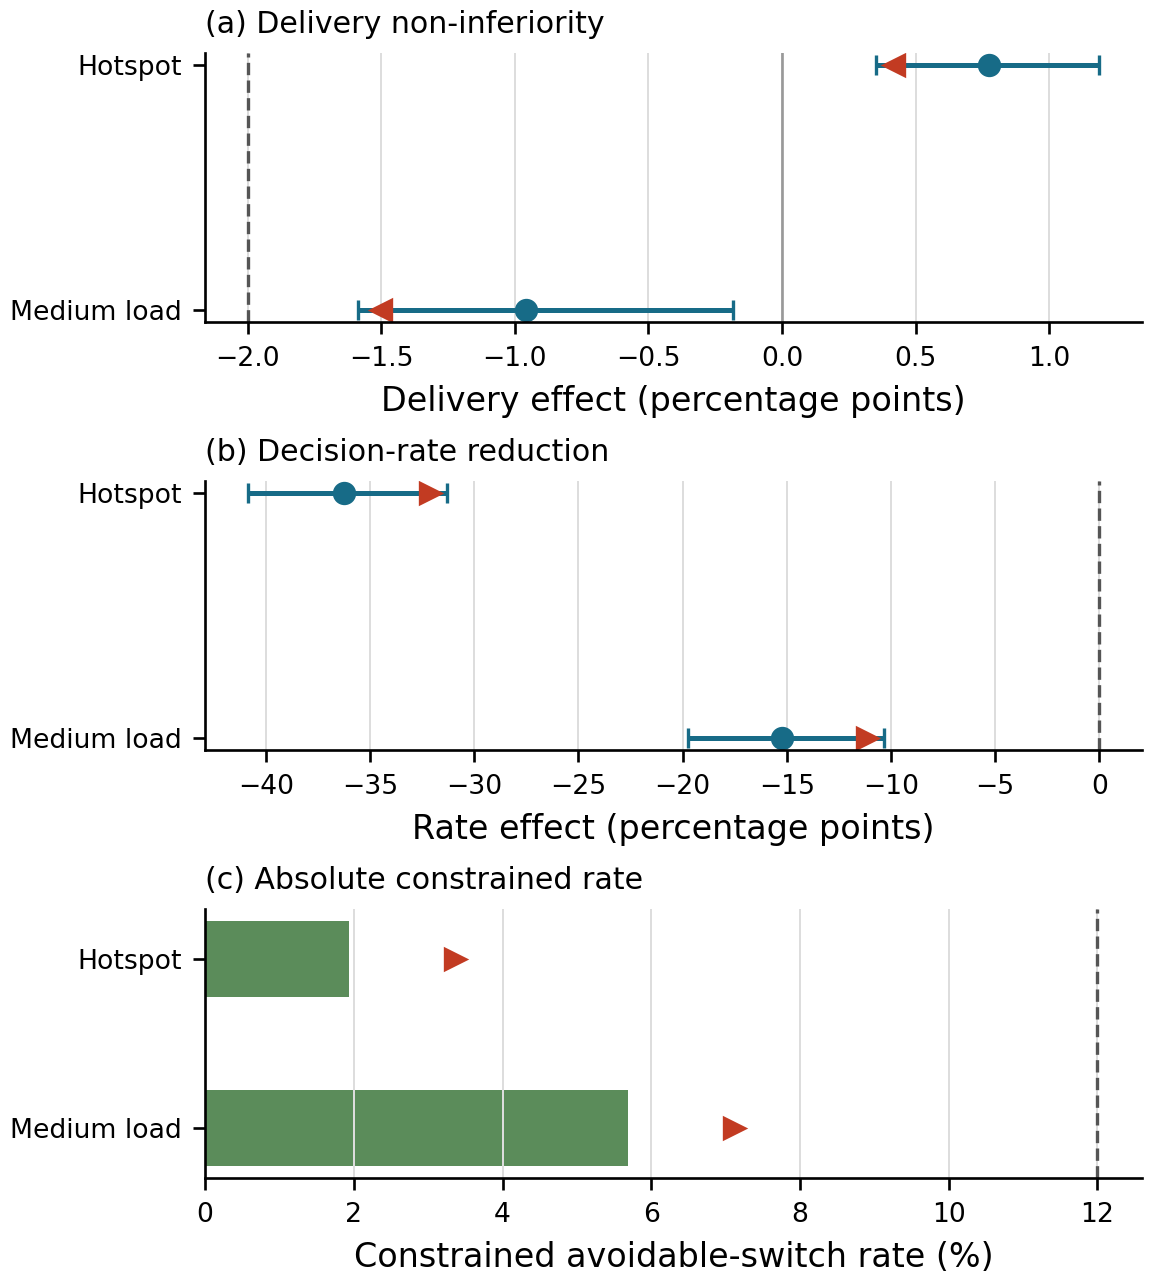
\includegraphics[width=\linewidth]{fig_sealed_results.png}
  \caption{Preregistered sealed-test effects. Bars are crossed-bootstrap 95\%
  intervals; triangles show one-sided 95\% gate bounds.}
  \label{fig:sealed}
\end{figure}

\begin{table}[t]
\centering
\caption{Sealed-Test Primary Results}
\scriptsize
\begin{tabular}{lrr}
\toprule
Metric & Medium & Hotspot\\
\midrule
Baseline delivery & 0.7925 & 0.2868\\
Constrained delivery & 0.7829 & 0.2945\\
Delivery effect (pp) & -0.958 & +0.772\\
95\% CI (pp) & [-1.587,-0.182] & [0.353,1.188]\\
One-sided lower (pp) & -1.503 & +0.419\\
Baseline switch rate & 0.2090 & 0.3818\\
Constrained switch rate & 0.0568 & 0.0194\\
Rate effect & -0.1522 & -0.3625\\
95\% CI & [-0.1974,-0.1036] & [-0.4087,-0.3130]\\
Maximum seed rate & 0.1091 & 0.0711\\
All gates & pass & pass\\
\bottomrule
\end{tabular}
\end{table}

Under medium load, the constraint reduced the rate from 0.2090 to 0.0568,
while delivery changed from 0.7925 to 0.7829. The one-sided delivery lower
bound was -1.503 percentage points, above the -2-point margin. Under hotspot
load, the rate fell from 0.3818 to 0.0194 and delivery increased by 0.772
points. Rate reductions were directionally consistent across all eight seeds
in both scenarios (raw exact $p=0.0078125$; Holm $p=0.03125$).

The constrained policy's medium-load delivery was close to Q-routing
(0.7829 versus 0.7875) and exceeded OSPF-ECMP and Global Dijkstra in this
simulator. In hotspot traffic, Q-routing delivered 0.3114 and the constrained
policy 0.2945. These classical comparisons are secondary and do not alter the
primary pass decision.

\section{Discussion and Limitations}
The result is a trade-off, not universal superiority. The medium-load policy
spends about one delivery point to remove most avoidable changes; hotspot
delivery improves relative to the matched unconstrained arm but remains below
Q-routing. The explicit constraint is materially more selective than scalar
reward shaping, whose rates were 0.1463 and 0.2427.

The evidence is limited to a synthetic 24-satellite slot simulator and two
traffic regimes. Local execution assumes fresh synchronous one-hop telemetry;
signaling cost, staleness, propagation delay, and packet-level protocol effects
are not modeled. The experiment supports neither throughput optimality nor
control-plane convergence. Generalization to larger constellations and
TLE/SGP4 or ns-3 traces remains future work.

\section{Conclusion}
An explicit decision-level constraint substantially reduced avoidable cached
next-hop changes while satisfying a prospective delivery non-inferiority rule
in both sealed scenarios. The candidate-set actor retains decentralized
execution and handles dynamic feasible actions. The frozen evaluation and
failure-visible reporting provide a reproducible basis for studying routing
stability beyond delivery-only optimization.

\begin{thebibliography}{9}
\bibitem{boyan1994q} J. Boyan and M. Littman, ``Packet routing in dynamically changing networks: A reinforcement learning approach,'' in \emph{NeurIPS}, 1994.
\bibitem{klenze2020hypatia} T. Klenze et al., ``Networking in heaven as on earth,'' in \emph{USENIX NSDI}, 2020.
\bibitem{zaheer2017deepsets} M. Zaheer et al., ``Deep sets,'' in \emph{NeurIPS}, 2017.
\bibitem{schulman2017ppo} J. Schulman et al., ``Proximal policy optimization algorithms,'' arXiv:1707.06347, 2017.
\bibitem{yu2022mappo} C. Yu et al., ``The surprising effectiveness of PPO in cooperative multi-agent games,'' in \emph{NeurIPS}, 2022.
\bibitem{velickovic2018gat} P. Veli\v{c}kovi\'c et al., ``Graph attention networks,'' in \emph{ICLR}, 2018.
\bibitem{henderson2018deep} P. Henderson et al., ``Deep reinforcement learning that matters,'' in \emph{AAAI}, 2018.
\bibitem{agarwal2021deep} R. Agarwal et al., ``Deep reinforcement learning at the edge of the statistical precipice,'' in \emph{NeurIPS}, 2021.
\end{thebibliography}
\end{document}
